\documentclass[../../main.tex]{subfiles}

\graphicspath{{../../image/}{../../figure/}}

\begin{document}

\section{主成分分析}\label{section:ch16-主成分分析}

主成分分析（PCA）已广泛应用于降维、有损数据压缩、特征提取和数据可视化等领域（Jolliffe, 2002），它也称为 Kosambi--Karhunen--Lo\`eve 变换。考虑将一个数据集正交投影到一个低维的线性空间[即主子空间（principal subspace）]，如\cref{figure:ch16-主子空间}所示。

\begin{figure}[htbp]
  \centering
  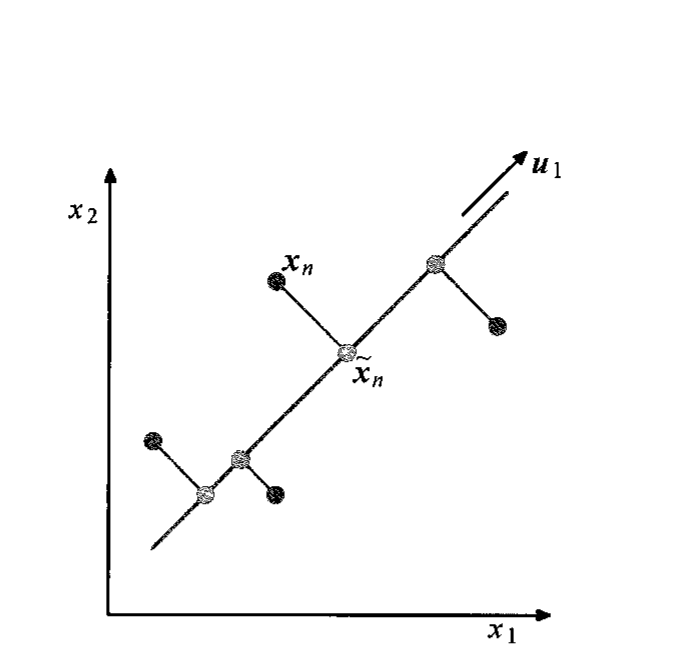
\includegraphics[width=0.52\textwidth]{ch16-fig16.2-principal-subspace.png}
  \caption{利用 PCA 寻求一个低维空间，称为主子空间（principal subspace），用洋红色线条表示，以使数据点（红色点）在主子空间中的正交投影能够最大化投影点（绿色点）的方差。PCA 的另一种定义是基于最小化投影误差的平方和给出的，这些误差用蓝色线条表示}
  \label{figure:ch16-主子空间}
\end{figure}

PCA 可以定义为最大化投影数据方差的线性投影（Hotelling, 1933）。同样，PCA 也可以定义为最小化平均投影代价的线性投影，平均投影代价则定义为数据点与其投影之间的均方距离（Pearson, 1901）。我们将依次学习这些定义。

\subsection{最大方差表述}\label{subsection:ch16-最大方差表述}

考虑一个观测数据集 $\{\bm{x}_n\}$，其中 $n=1,\cdots,N$，并且 $\bm{x}_n$ 是一个维度为 $D$ 的欧几里得变量。我们想要把数据投影到维度为 $M<D$ 的空间，同时最大化投影数据的方差。目前我们假设 $M$ 的值是给定的。在本章的后面，我们会学习从数据中确定 $M$ 的合适值的技术。

首先考虑投影到一维空间（$M=1$）。我们可以使用一个 $D$ 维向量 $\bm{u}_1$ 来定义这个空间的方向，为了方便（且不失一般性），我们会选择单位向量，因此 $\bm{u}_1^{\mathsf T}\bm{u}_1=1$（注意我们只对 $\bm{u}_1$ 定义的方向感兴趣）。然后将每个数据点 $\bm{x}_n$ 投影到一个标量值 $\bm{u}_1^{\mathsf T}\bm{x}_n$ 上。投影数据的平均值是 $\bm{u}_1^{\mathsf T}\bar{\bm{x}}$，其中 $\bar{\bm{x}}$ 是样本集的平均值，由下式给出：
\begin{align}
  \bar{\bm{x}}=\frac{1}{N}\sum_{n=1}^{N}\bm{x}_n.
  \label{align:ch16-均值}
\end{align}

投影数据的方差由下式给出：
\begin{align}
  \frac{1}{N}\sum_{n=1}^{N}\left\{\bm{u}_1^{\mathsf T}\bm{x}_n-\bm{u}_1^{\mathsf T}\bar{\bm{x}}\right\}^2=\bm{u}_1^{\mathsf T}\bm{S}\bm{u}_1,
  \label{align:ch16-投影方差}
\end{align}
其中 $\bm{S}$ 是数据协方差矩阵，定义为
\begin{align}
  \bm{S}=\frac{1}{N}\sum_{n=1}^{N}(\bm{x}_n-\bar{\bm{x}})(\bm{x}_n-\bar{\bm{x}})^{\mathsf T}.
  \label{align:ch16-协方差}
\end{align}

下面我们将投影数据的方差 $\bm{u}_1^{\mathsf T}\bm{S}\bm{u}_1$ 相对于 $\bm{u}_1$ 最大化。显然，这必须是一个受约束的最大化操作，以防止 $\|\bm{u}_1\|\rightarrow\infty$。适当的约束来源于归一化条件 $\bm{u}_1^{\mathsf T}\bm{u}_1=1$。为了强制执行这个约束，我们引入一个 Lagrange 乘子（见\hyperref[chapter:appC-Lagrange乘子]{附录\ref*{chapter:appC-Lagrange乘子}}），记作 $\lambda_1$，并对下式进行无约束的最大化：
\begin{align}
  \bm{u}_1^{\mathsf T}\bm{S}\bm{u}_1+\lambda_1(1-\bm{u}_1^{\mathsf T}\bm{u}_1).
  \label{align:ch16-Lagrange}
\end{align}

通过将\eqref{align:ch16-Lagrange}对 $\bm{u}_1$ 的导数设为零，我们发现当以下条件满足时，目标函数将取驻点：
\begin{align}
  \bm{S}\bm{u}_1=\lambda_1\bm{u}_1.
  \label{align:ch16-特征方程}
\end{align}

这意味着 $\bm{u}_1$ 必须是 $\bm{S}$ 的一个特征向量。如果将\eqref{align:ch16-特征方程}左乘 $\bm{u}_1^{\mathsf T}$ 并利用归一化条件 $\bm{u}_1^{\mathsf T}\bm{u}_1=1$，可得方差为
\begin{align}
  \bm{u}_1^{\mathsf T}\bm{S}\bm{u}_1=\lambda_1.
  \label{align:ch16-特征值方差}
\end{align}

因此，当我们将 $\bm{u}_1$ 设置为具有最大特征值 $\lambda_1$ 的特征向量时，方差将达到最大。

\begin{definition}[主成分与主子空间]\label{definition:ch16-主成分}
设 $\bm{S}$ 是数据集的 $D\times D$ 协方差矩阵，其特征值为 $\lambda_1\geqslant\lambda_2\geqslant\cdots\geqslant\lambda_D$，对应的单位特征向量为 $\bm{u}_1,\cdots,\bm{u}_D$。称对应于最大特征值的特征向量 $\bm{u}_1$ 为第一主成分（first principal component）。一般地，在 $\bm{u}_1,\cdots,\bm{u}_{M-1}$ 已经选定之后，称在所有与它们正交的单位向量中使投影方差 $\bm{u}^{\mathsf T}\bm{S}\bm{u}$ 取最大值的 $\bm{u}_M$ 为第 $M$ 个主成分，称由前 $M$ 个主成分张成的 $M$ 维线性子空间为主子空间（principal subspace）。
\end{definition}

% SUPPLEMENT: parent=definition:ch16-主成分; kind=motivation; location=紧随其后的 remark（重构新增）
\begin{remark}（重构新增）
PCA 要解决的问题是：在 $D$ 维数据空间中找出一个 $M$ 维线性子空间，使得把数据压缩到该子空间上所丢失的信息尽可能少。这里把“信息”量化为投影后数据的方差，理由是：若某个方向上的投影几乎没有变化，那么沿该方向的坐标对区分数据点毫无贡献，删去它不会损失可分性；反之，投影方差大的方向保留了数据的主要变动。因此“最大化投影方差”是对“保留最多信息”的一种可计算的具体化。

定义中的几个条件各有作用。第一，归一化约束 $\bm{u}_1^{\mathsf T}\bm{u}_1=1$ 不是数学上的限制而是必要的：若不加约束，$\bm{u}_1^{\mathsf T}\bm{S}\bm{u}_1$ 可以沿任一使二次型取正的方向无限增大，最大化问题没有解；归一化把可行集变成紧集（单位球面），从而最大值一定取到。第二，$M$ 被当作给定常数，是因为主成分的个数是模型选择问题，本书后面会用 Bayes 方法从数据中确定它；此处先假定已知，以免与优化问题混在一起。第三，协方差矩阵 $\bm{S}$ 对称半正定，故其特征值非负且可取正交特征向量组，这是\eqref{align:ch16-特征方程}有实解并可按大小排序的前提。此外，$\bm{S}$ 采用除以 $N$ 的约定，除以 $N-1$ 的无偏估计只与之相差一个常数因子，不影响特征向量的结论。
\end{remark}

我们可以通过逐步的方式定义更多的主成分，方法就是选取一个新方向，使其在所有与已考虑方向正交的方向中最大化投影后的方差。考虑 $M$ 维投影空间的一般情况，投影数据方差最大化的最优线性投影由数据协方差矩阵 $\bm{S}$ 对应于最大特征值 $\lambda_1,\cdots,\lambda_M$ 的 $M$ 个特征向量 $\bm{u}_1,\cdots,\bm{u}_M$ 定义（见\cref{exercise:ch16-01}）。这可以很容易地使用数学归纳法来证明。

\begin{proposition}[最大方差表述的最优性]\label{proposition:ch16-最大方差}
设 $\bm{S}$ 为 $D\times D$ 对称半正定矩阵，其特征值按 $\lambda_1\geqslant\cdots\geqslant\lambda_D\geqslant0$ 排列，对应的单位特征向量为 $\bm{u}_1,\cdots,\bm{u}_D$ 且两两正交。对任意 $1\leqslant M\leqslant D$，在全体满足 $\bm{u}_i^{\mathsf T}\bm{u}_j=\delta_{ij}$ 的 $D$ 维向量组 $\{\bm{u}_1,\cdots,\bm{u}_M\}$ 上，投影数据的方差之和
\begin{align*}
  \sum_{i=1}^{M}\bm{u}_i^{\mathsf T}\bm{S}\bm{u}_i
\end{align*}
的最大值等于 $\sum_{i=1}^{M}\lambda_i$，且当且仅当 $\{\bm{u}_1,\cdots,\bm{u}_M\}$ 张成由前 $M$ 个特征向量张成的子空间时取到。
\end{proposition}

\begin{proof}（重构新增）
对 $M$ 作归纳。$M=1$ 的情形已由\eqref{align:ch16-特征方程}与\eqref{align:ch16-特征值方差}给出：单位球面是紧集，$\bm{u}^{\mathsf T}\bm{S}\bm{u}$ 连续，故最大值存在；在约束 $\bm{u}^{\mathsf T}\bm{u}=1$ 下用乘子 $\lambda$，驻点满足 $\bm{S}\bm{u}=\lambda\bm{u}$，代回得目标值 $\lambda$，故最大值是最大特征值 $\lambda_1$，在 $\bm{u}=\bm{u}_1$（或其反向）处取到。

设结论对 $M-1$ 成立，即 $\bm{u}_1,\cdots,\bm{u}_{M-1}$ 必须张成前 $M-1$ 个特征向量张成的子空间 $\mathcal{U}_{M-1}$，此时方差之和为 $\sum_{i=1}^{M-1}\lambda_i$。现在固定这一部分，只对 $\bm{u}_M$ 优化，约束为
\begin{align*}
  \bm{u}_M^{\mathsf T}\bm{u}_M=1,\qquad \bm{u}_M^{\mathsf T}\bm{u}_j=0\quad(j=1,\cdots,M-1).
\end{align*}
引入乘子 $\lambda$ 与 $\mu_1,\cdots,\mu_{M-1}$，对下式求驻点：
\begin{align*}
  \tilde{J}=\bm{u}_M^{\mathsf T}\bm{S}\bm{u}_M+\lambda(1-\bm{u}_M^{\mathsf T}\bm{u}_M)+\sum_{j=1}^{M-1}\mu_j\bm{u}_M^{\mathsf T}\bm{u}_j .
\end{align*}
对 $\bm{u}_M$ 求导并令其为零，得
\begin{align*}
  2\bm{S}\bm{u}_M-2\lambda\bm{u}_M+\sum_{j=1}^{M-1}\mu_j\bm{u}_j=\bm{0}.
\end{align*}
左乘 $\bm{u}_k^{\mathsf T}$（$k\leqslant M-1$），利用 $\bm{u}_M^{\mathsf T}\bm{u}_k=0$ 与 $\bm{u}_j^{\mathsf T}\bm{u}_k=\delta_{jk}$，得 $2\bm{u}_k^{\mathsf T}\bm{S}\bm{u}_M+\mu_k=0$。由于 $\bm{u}_k$ 是 $\bm{S}$ 的特征向量，$\bm{u}_k^{\mathsf T}\bm{S}\bm{u}_M=\lambda_k\bm{u}_k^{\mathsf T}\bm{u}_M=0$，故 $\mu_k=0$。于是驻点方程退化为 $\bm{S}\bm{u}_M=\lambda\bm{u}_M$：$\bm{u}_M$ 是 $\bm{S}$ 的特征向量，且与 $\mathcal{U}_{M-1}$ 正交，因此它必是 $\bm{u}_M,\cdots,\bm{u}_D$ 之一，相应的目标值为其特征值。在剩下的特征值 $\lambda_M\geqslant\cdots\geqslant\lambda_D$ 中取最大者，即得 $\bm{u}_M=\bm{u}_{M+1}$ 之前的那一个，也就是 $\bm{u}_M$，目标值为 $\lambda_M$。故 $M$ 时的最大值为 $\sum_{i=1}^{M}\lambda_i$。

唯一性：若某个最优解张成的子空间与 $\mathcal{U}_M$ 不同，则它对应的特征值之和不可能是最大的 $M$ 个（除非出现重特征值，此时不同的特征向量组合张成同一子空间，命题所说的“张成”仍然成立）。因此最优解在子空间意义下唯一。
\end{proof}

% SUPPLEMENT: parent=proposition:ch16-最大方差; kind=motivation; location=紧随其后的 remark（重构新增）
\begin{remark}（重构新增）
本命题把“逐步选取正交方向”这一构造提升为全局最优性断言：不必逐个求解 $M$ 次约束优化，只需对 $\bm{S}$ 作一次特征分解，取最大的 $M$ 个特征值对应的特征向量即可。证明的关键是：在已取定前 $M-1$ 个方向后，新方向对旧方向的乘子全部为零，因为旧方向本身就是 $\bm{S}$ 的特征向量、与任何候选新方向正交；这一点使问题逐层解耦。

条件的作用如下。$\bm{S}$ 的对称性是“特征向量可取为正交组”的来源；半正定性保证 $\lambda_i\geqslant0$，从而“取最大的特征值”等价于“取最大的方差”。若 $\bm{S}$ 有重特征值，则对应的特征向量不唯一，但张成的子空间唯一，命题的结论仍成立；此时主成分子空间仍然良定义，只是单个主成分的方向不唯一。若去掉正交约束，问题会退化：各 $\bm{u}_i$ 都取同一个最大特征向量时方差之和为 $M\lambda_1$，这并没有给出 $M$ 个不同的方向，故正交约束是必要的。
\end{remark}

综上，PCA 涉及计算数据集的均值 $\bar{\bm{x}}$ 和数据协方差矩阵 $\bm{S}$，然后找到 $\bm{S}$ 对应于最大特征值的 $M$ 个特征向量。关于寻找特征向量和特征值的算法，以及与特征向量分解相关的附加定理，可以在 Golub and Van Loan (1996) 中找到。请注意，计算一个 $D\times D$ 大小矩阵的完整特征向量分解的计算成本是 $\mathcal{O}(D^3)$。如果打算将数据投影到前 $M$ 个主成分上，则只需要找到前 $M$ 个特征值和特征向量。这可以通过使用更有效的方法来完成，比如幂方法（Golub and Van Loan, 1996），复杂度为 $\mathcal{O}(MD^2)$，当然也可以使用 EM 算法（见\cref{subsection:ch16-PCA的EM算法}）。

\subsection{最小误差表述}\label{subsection:ch16-最小误差表述}

本小节讨论基于投影误差最小化的 PCA 的另一种表述（见\hyperref[chapter:appA-线性代数]{附录\ref*{chapter:appA-线性代数}}）。为此，引入一组 $D$ 维的完备正交规范的基向量 $\{\bm{u}_i\}$，其中 $i=1,\cdots,D$，它们满足
\begin{align}
  \bm{u}_i^{\mathsf T}\bm{u}_j=\delta_{ij}.
  \label{align:ch16-正交基}
\end{align}

由于这组基向量是完备的，每个数据点都可以通过基向量的线性组合精确表示为
\begin{align}
  \bm{x}_n=\sum_{i=1}^{D}\alpha_{ni}\bm{u}_i,
  \label{align:ch16-基展开}
\end{align}
其中系数 $\alpha_{ni}$ 对于不同的数据点是不同的。这只是相当于将坐标系旋转到 $\{\bm{u}_i\}$ 定义的新系统，原始的 $D$ 个分量 $\{x_{n1},\cdots,x_{nD}\}$ 被等价的一组分量 $\{\alpha_{n1},\cdots,\alpha_{nD}\}$ 替代。与 $\bm{u}_j$ 内积并利用正交性质，可以得到 $\alpha_{nj}=\bm{x}_n^{\mathsf T}\bm{u}_j$。因此，不失一般性地，我们可以写作
\begin{align}
  \bm{x}_n=\sum_{i=1}^{D}\left(\bm{x}_n^{\mathsf T}\bm{u}_i\right)\bm{u}_i.
  \label{align:ch16-系数}
\end{align}

不过，我们的目标是用一个较小的变量数 $M$（小于原始维度 $D$）来近似这个数据点，相当于将它投影到一个低维的子空间。这个 $M$ 维的线性子空间可以用前 $M$ 个基向量表示，这样我们就可以用这些基向量来近似每一个数据点 $\bm{x}_n$：
\begin{align}
  \tilde{\bm{x}}_n=\sum_{i=1}^{M}z_{ni}\bm{u}_i+\sum_{i=M+1}^{D}b_i\bm{u}_i,
  \label{align:ch16-近似}
\end{align}
其中 $\{z_{ni}\}$ 依赖于特定的数据点，而 $\{b_i\}$ 是对所有数据点都相同的常数。我们可以自由选择 $\{\bm{u}_i\}$、$\{z_{ni}\}$ 和 $\{b_i\}$，以最小化由维度降低引入的误差。

作为误差度量，我们将使用原始数据点 $\bm{x}_n$ 与其近似值 $\tilde{\bm{x}}_n$ 之间的平方距离，并在数据集上取平均，因此我们的目标是最小化
\begin{align}
  J=\frac{1}{N}\sum_{n=1}^{N}\|\bm{x}_n-\tilde{\bm{x}}_n\|^2.
  \label{align:ch16-重建误差}
\end{align}

首先考虑关于量 $\{z_{ni}\}$ 的最小化。将 $\tilde{\bm{x}}_n$ 代入 $J$，将 $J$ 关于 $z_{ni}$ 的导数设为零，利用正交关系，我们得到
\begin{align}
  z_{ni}=\bm{x}_n^{\mathsf T}\bm{u}_i,
  \label{align:ch16-z最优}
\end{align}
其中 $i=1,\cdots,M$。类似地，将 $J$ 关于 $b_i$ 的导数设为零，并再次利用正交关系，得到
\begin{align}
  b_i=\bar{\bm{x}}^{\mathsf T}\bm{u}_i,
  \label{align:ch16-b最优}
\end{align}
其中 $i=M+1,\cdots,D$。代入 $z_{ni}$ 和 $b_i$，并利用一般展开式[\eqref{align:ch16-系数}]，得到
\begin{align}
  \bm{x}_n-\tilde{\bm{x}}_n=\sum_{i=M+1}^{D}\left\{(\bm{x}_n-\bar{\bm{x}})^{\mathsf T}\bm{u}_i\right\}\bm{u}_i.
  \label{align:ch16-残差}
\end{align}

我们看到，从 $\bm{x}_n$ 到 $\tilde{\bm{x}}_n$ 的位移向量位于主子空间的正交空间中，因为它是 $i=M+1,\cdots,D$ 的 $\bm{u}_i$ 的线性组合，如\cref{figure:ch16-主子空间}所示。这在预期之内，因为投影点 $\tilde{\bm{x}}_n$ 必须位于主子空间内，但我们可以在这个子空间内自由移动它们，因此最小误差由正交投影给出。

在考虑正式的解之前，让我们通过一个二维的特例来直观地理解 $J$ 的最小化。

\begin{example}[ 二维数据的一维主子空间]\label{example:ch16-二维主成分}
考虑二维数据空间（$D=2$）与一维主子空间（$M=1$）。此时误差度量只涉及一个方向 $\bm{u}_2$，且约束为正交归一条件 $\bm{u}_2^{\mathsf T}\bm{u}_2=1$。以乘子 $\lambda_2$ 强制该约束，考虑最小化
\begin{align}
  \tilde{J}=\bm{u}_2^{\mathsf T}\bm{S}\bm{u}_2+\lambda_2\left(1-\bm{u}_2^{\mathsf T}\bm{u}_2\right).
  \label{align:ch16-误差Lagrange}
\end{align}
将 $\tilde{J}$ 关于 $\bm{u}_2$ 的导数设为零，得到 $\bm{S}\bm{u}_2=\lambda_2\bm{u}_2$，即 $\bm{u}_2$ 是 $\bm{S}$ 的一个特征向量，具有特征值 $\lambda_2$。因此，任何特征向量都将定义误差度量的驻点。要找到 $J$ 在最小值点的值，可以将方程对 $\bm{u}_2$ 的解回代到误差度量中，得到 $J=\lambda_2$。因此，我们可以通过选择 $\bm{u}_2$ 为对应于两个特征值中较小的那个特征向量来获得 $J$ 的最小值。我们应该选择让主成分子空间与具有较大特征值的特征向量对齐。这个结果符合我们的直觉，即为了最小化平均平方投影距离，应该选择主成分子空间，使其通过数据点的平均值并与最大方差的方向对齐。只要特征值相等，任何选择的主方向都将产生相同的 $J$ 值。
\end{example}

\begin{remark}（重构新增）
这个二维例子把一般情形中的两个量分离清楚了：$J$ 的驻点条件与最大方差表述的驻点条件是同一个特征方程，区别只在于目标函数是 $\bm{u}^{\mathsf T}\bm{S}\bm{u}$ 还是它的相反数，因此驻点集合相同，而“取最大”与“取最小”的差别就体现为选最大还是最小的特征值。这正是两种表述等价的直观来源。当两个特征值相等时，$\bm{S}$ 是单位矩阵的倍数，所有方向的投影误差都相同，$J$ 与方向无关，这与“任何选择的主方向都产生相同的 $J$”一致。
\end{remark}

误差度量 $J$ 作为纯粹依赖于 $\{\bm{u}_i\}$ 的函数的表达式如下：
\begin{align}
  J=\frac{1}{N}\sum_{n=1}^{N}\sum_{i=M+1}^{D}\left(\bm{x}_n^{\mathsf T}\bm{u}_i-\bar{\bm{x}}^{\mathsf T}\bm{u}_i\right)^2=\sum_{i=M+1}^{D}\bm{u}_i^{\mathsf T}\bm{S}\bm{u}_i.
  \label{align:ch16-误差函数}
\end{align}

剩下的任务是调整 $\{\bm{u}_i\}$ 从而最小化 $J$，这也必须是一个受约束的最小化操作，否则我们将得到毫无意义的结果 $\bm{u}_i=\bm{0}$。约束来源于正交条件，正如我们将看到的，解将以协方差矩阵的特征向量的形式表示出来。

针对任意 $D$ 和任意 $M<D$ 最小化 $J$ 的一般解，均可以选择 $\bm{u}_i$ 为协方差矩阵的特征向量（见\cref{exercise:ch16-02}），由下式给出：
\begin{align}
  \bm{S}\bm{u}_i=\lambda_i\bm{u}_i,
  \label{align:ch16-特征方程全}
\end{align}
其中 $i=1,\cdots,D$，并且像往常一样，特征向量 $\bm{u}_i$ 选择为正交向量。然后，误差度量的相应值由下式给出：
\begin{align}
  J=\sum_{i=M+1}^{D}\lambda_i.
  \label{align:ch16-误差最小值}
\end{align}

\begin{proposition}[最小误差表述与最大方差表述的等价性]\label{proposition:ch16-最小误差}
设 $\bm{S}$ 为 $D\times D$ 对称半正定矩阵，特征值按 $\lambda_1\geqslant\cdots\geqslant\lambda_D\geqslant0$ 排列。在 $\tilde{\bm{x}}_n$ 由\eqref{align:ch16-近似}给出、$\{\bm{u}_i\}$ 满足\eqref{align:ch16-正交基}的条件下，误差度量 $J$ 的最小值为 $\sum_{i=M+1}^{D}\lambda_i$，且最小值在 $\bm{u}_1,\cdots,\bm{u}_M$ 张成前 $M$ 个特征向量张成的子空间时取到；换言之，最小误差表述与\cref{proposition:ch16-最大方差}的最大方差表述给出同一个主子空间。
\end{proposition}

\begin{proof}（重构新增）
第一步，关于系数的最优化。把\eqref{align:ch16-近似}代入\eqref{align:ch16-重建误差}，并利用\eqref{align:ch16-正交基}展开范数：
\begin{align*}
  J=\frac{1}{N}\sum_{n=1}^{N}\left\{\sum_{i=1}^{M}\left(z_{ni}-\bm{x}_n^{\mathsf T}\bm{u}_i\right)^2+\sum_{i=M+1}^{D}\left(b_i-\bm{x}_n^{\mathsf T}\bm{u}_i\right)^2\right\}.
\end{align*}
右端关于 $z_{ni}$ 与 $b_i$ 分别是独立的二次函数，逐项配方即知最小值在 $z_{ni}=\bm{x}_n^{\mathsf T}\bm{u}_i$ 与 $b_i=\frac{1}{N}\sum_n\bm{x}_n^{\mathsf T}\bm{u}_i=\bar{\bm{x}}^{\mathsf T}\bm{u}_i$ 处取到，这正是\eqref{align:ch16-z最优}与\eqref{align:ch16-b最优}；此时每个平方项为零，$J$ 只剩下被丢弃的分量，即\eqref{align:ch16-残差}与\eqref{align:ch16-误差函数}。

第二步，关于基的最优化。由\eqref{align:ch16-误差函数}，记 $\tilde{\bm{U}}$ 为以 $\bm{u}_{M+1},\cdots,\bm{u}_D$ 为列的 $D\times(D-M)$ 矩阵，则 $J=\operatorname{tr}(\tilde{\bm{U}}^{\mathsf T}\bm{S}\tilde{\bm{U}})$，约束为 $\tilde{\bm{U}}^{\mathsf T}\tilde{\bm{U}}=\bm{I}$（即\eqref{align:ch16-正交基}中 $i,j>M$ 的部分）。引入对称乘子矩阵 $\bm{H}$，考虑
\begin{align}
  \tilde{J}=\operatorname{tr}\left[\tilde{\bm{U}}^{\mathsf T}\bm{S}\tilde{\bm{U}}\right]+\operatorname{tr}\left[\bm{H}\left(\bm{I}-\tilde{\bm{U}}^{\mathsf T}\tilde{\bm{U}}\right)\right].
  \label{align:ch16-误差矩阵形式}
\end{align}
（约束矩阵 $\bm{I}-\tilde{\bm{U}}^{\mathsf T}\tilde{\bm{U}}$ 对称，故只需 $\bm{H}$ 的对称部分，可设 $\bm{H}$ 对称。）关于 $\tilde{\bm{U}}$ 求导并令其为零，得
\begin{align*}
  \bm{S}\tilde{\bm{U}}=\tilde{\bm{U}}\bm{H}.
\end{align*}
由于 $\bm{H}$ 对称，存在正交矩阵 $\bm{V}$ 使 $\bm{V}^{\mathsf T}\bm{H}\bm{V}=\bm{\Lambda}'$ 为对角矩阵。右乘 $\bm{V}$ 得 $\bm{S}(\tilde{\bm{U}}\bm{V})=(\tilde{\bm{U}}\bm{V})\bm{\Lambda}'$。又 $\tilde{\bm{U}}\bm{V}$ 的列仍两两正交且为单位向量，故不妨设 $\tilde{\bm{U}}$ 的列就是 $\bm{S}$ 的特征向量；此时 $\bm{H}=\tilde{\bm{U}}^{\mathsf T}\bm{S}\tilde{\bm{U}}=\bm{\Lambda}'$，$J=\operatorname{tr}(\bm{H})$ 等于所选 $D-M$ 个特征值之和。

第三步，取最小的 $D-M$ 个特征值 $\lambda_{M+1},\cdots,\lambda_D$ 即得 $J=\sum_{i=M+1}^{D}\lambda_i$，这就是 $J$ 的最小值；相应地，主子空间由剩下的 $M$ 个特征向量 $\bm{u}_1,\cdots,\bm{u}_M$ 张成，即前 $M$ 个最大特征值对应的特征向量张成的子空间。把它与\cref{proposition:ch16-最大方差}对照：那里最大化的正是 $\sum_{i=1}^{M}\bm{u}_i^{\mathsf T}\bm{S}\bm{u}_i$，而这里 $J=\sum_{i=M+1}^{D}\bm{u}_i^{\mathsf T}\bm{S}\bm{u}_i=\operatorname{tr}(\bm{S})-\sum_{i=1}^{M}\bm{u}_i^{\mathsf T}\bm{S}\bm{u}_i$（因为 $\{\bm{u}_i\}$ 是完备正交基，$\operatorname{tr}(\bm{S})=\sum_{i=1}^{D}\bm{u}_i^{\mathsf T}\bm{S}\bm{u}_i$）。由于 $\operatorname{tr}(\bm{S})$ 与基的选取无关，最小化 $J$ 与最大化前 $M$ 项之和是同一个问题，两者的最优子空间相同。
\end{proof}

% SUPPLEMENT: parent=proposition:ch16-最小误差; kind=motivation; location=紧随其后的 remark（重构新增）
\begin{remark}（重构新增）
本命题说明 PCA 的两种经典表述——Hotelling 的最大方差表述与 Pearson 的最小误差表述——在最优化意义下完全等价，因此可以按计算上的方便任选其一。证明中真正起作用的结构是：$\{\bm{u}_i\}$ 是完备正交基，于是迹可分解为两部分，而被丢弃的那部分恰是 $J$。这条恒等式 $\operatorname{tr}(\bm{S})=\sum_{i}\bm{u}_i^{\mathsf T}\bm{S}\bm{u}_i$ 依赖正交归一条件\eqref{align:ch16-正交基}；若基不正交，交叉项不会消失，$J$ 就不再等于 $\operatorname{tr}(\bm{S})$ 减去保留部分，两种表述的等价性也随之失效。

需要强调的是，“$J$ 的最小值为 $\sum_{i=M+1}^{D}\lambda_i$”这一结论中特征值必须按降序排列；若把最小的特征值排在前面，公式本身仍然成立，但“主子空间由前 $M$ 个特征向量张成”的说法就要改成“由最大的 $M$ 个特征值对应的特征向量张成”。此外，$\lambda_i$ 是投影误差的逐方向贡献，因此\eqref{align:ch16-误差最小值}也给出了选择 $M$ 的定量依据：当 $\lambda_{M+1},\cdots,\lambda_D$ 相对于 $\lambda_1,\cdots,\lambda_M$ 很小时，取 $M$ 维主子空间的误差可以忽略。
\end{remark}

这仅仅是正交于主子空间的那些特征向量的特征值之和。因此，我们通过选择这些特征向量为具有 $D-M$ 个最小特征值的那些特征向量，得到了 $J$ 的最小值，定义主子空间的特征向量是对应于 $M$ 个最大特征值的那些特征向量。这个结果符合我们的直觉：为了最小化平均平方投影距离，应该选择主成分子空间，使其通过数据点的平均值并与最大方差的方向对齐。

虽然我们仅考虑了 $M<D$ 的情况，但如果 $M=D$，PCA 仍然成立，在这种情况下没有降维，只是简单地旋转坐标轴以与主成分对齐。

最后请注意，有一种相关的线性降维技术称为典型相关分析（Canonical Correlation Analysis, CCA）（Hotelling, 1936; Bach and Jordan, 2002）。PCA 只处理单个随机变量，而典型相关分析则考虑多个变量，并尝试找到具有高度互相关性的对应线性子空间对，以使一个子空间内的分量与另一个子空间内的分量具有相关性。它的解可以用广义特征向量问题来表示。

\subsection{数据压缩}\label{subsection:ch16-数据压缩}

PCA 的另一个应用是数据压缩，我们用手写数字图像数据集来举例。因为协方差矩阵的每个特征向量都是原始 $D$ 维空间中的向量，所以我们可以将特征向量表示成与数据点大小相同的图像。平均向量和前 $4$ 个 PCA 特征向量及对应的特征值如\cref{figure:ch16-PCA特征向量}所示。

\begin{figure}[htbp]
  \centering
  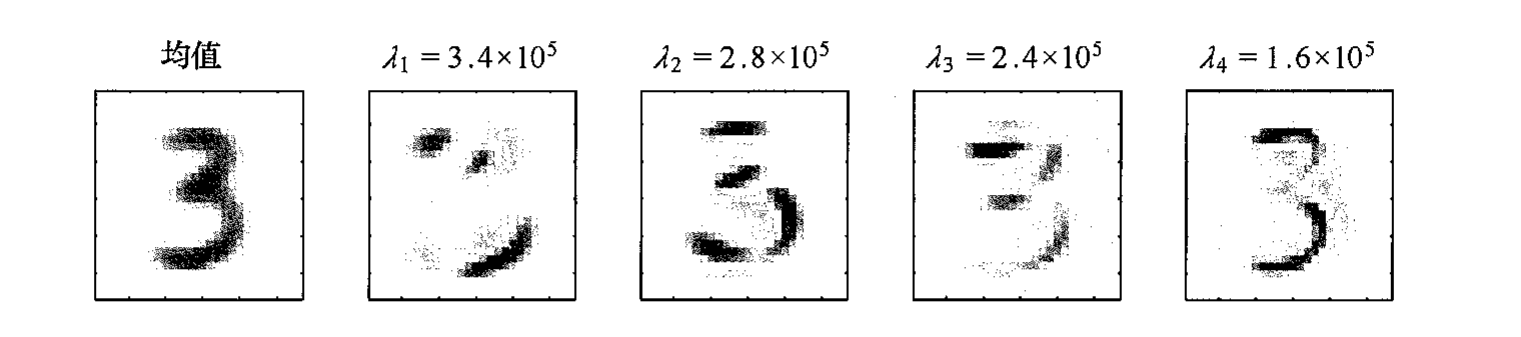
\includegraphics[width=0.95\textwidth]{ch16-fig16.3-pca-eigenvectors.png}
  \caption{将 PCA 应用于一个由 6000 个 $28\times28$ 像素的手写数字“3”的图像数据集，这里展现了平均向量 $\bar{\bm{x}}$ 和前 4 个 PCA 特征向量 $\bm{u}_1,\cdots,\bm{u}_4$ 及对应的特征值}
  \label{figure:ch16-PCA特征向量}
\end{figure}

完整特征值谱的排序递减图如\cref{figure:ch16-特征值谱}中的 (a) 所示。与选择特定的 $M$ 值相关联的误差度量 $J$ 由第 $M+1$ 到第 $D$ 个特征值的和给出，并且不同 $M$ 值的情况已绘制在同一图的 (b) 中。

\begin{figure}[htbp]
  \centering
  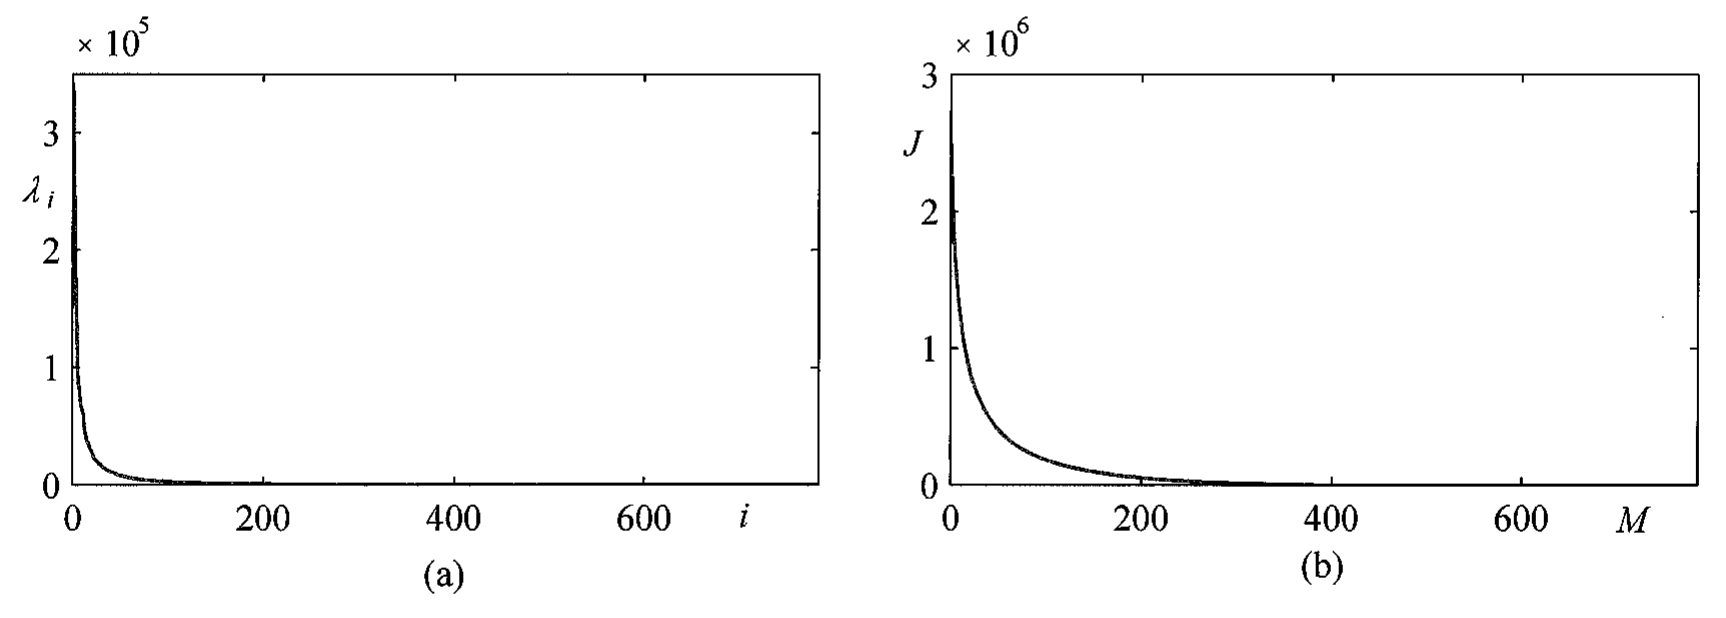
\includegraphics[width=0.95\textwidth]{ch16-fig16.4-eigenvalue-spectrum.png}
  \caption{(a) \cref{figure:ch16-PCA特征向量}中使用的手写数字图像数据集的特征值谱图；(b) 被抛弃特征值的和代表了通过将数据投影到维度为 $M$ 的主子空间而引入的平方和误差 $J$}
  \label{figure:ch16-特征值谱}
\end{figure}

如果我们将在\eqref{align:ch16-z最优}和\eqref{align:ch16-b最优}代入\eqref{align:ch16-近似}，就可以将 PCA 近似于数据向量 $\bm{x}_n$ 的形式写为
\begin{align}
  \tilde{\bm{x}}_n&=\sum_{i=1}^{M}\left(\bm{x}_n^{\mathsf T}\bm{u}_i\right)\bm{u}_i+\sum_{i=M+1}^{D}\left(\bar{\bm{x}}^{\mathsf T}\bm{u}_i\right)\bm{u}_i\nonumber\\
  &=\bar{\bm{x}}+\sum_{i=1}^{M}\left(\bm{x}_n^{\mathsf T}\bm{u}_i-\bar{\bm{x}}^{\mathsf T}\bm{u}_i\right)\bm{u}_i,
  \label{align:ch16-重建}
\end{align}
其中我们利用了如下关系：
\begin{align}
  \bar{\bm{x}}=\sum_{i=1}^{D}\left(\bar{\bm{x}}^{\mathsf T}\bm{u}_i\right)\bm{u}_i.
  \label{align:ch16-均值展开}
\end{align}

式\eqref{align:ch16-均值展开}成立是因为 $\{\bm{u}_i\}$ 的完备性。这代表了数据集的压缩，因为对于每个数据点，我们都会将 $D$ 维向量 $\bm{x}_n$ 替换为具有分量 $(\bm{x}_n^{\mathsf T}\bm{u}_i-\bar{\bm{x}}^{\mathsf T}\bm{u}_i)$ 的 $M$ 维向量。$M$ 值越小，压缩程度越大。手写数字图像数据集的 PCA 重建数据点示例见\cref{figure:ch16-PCA重建}。

\begin{figure}[htbp]
  \centering
  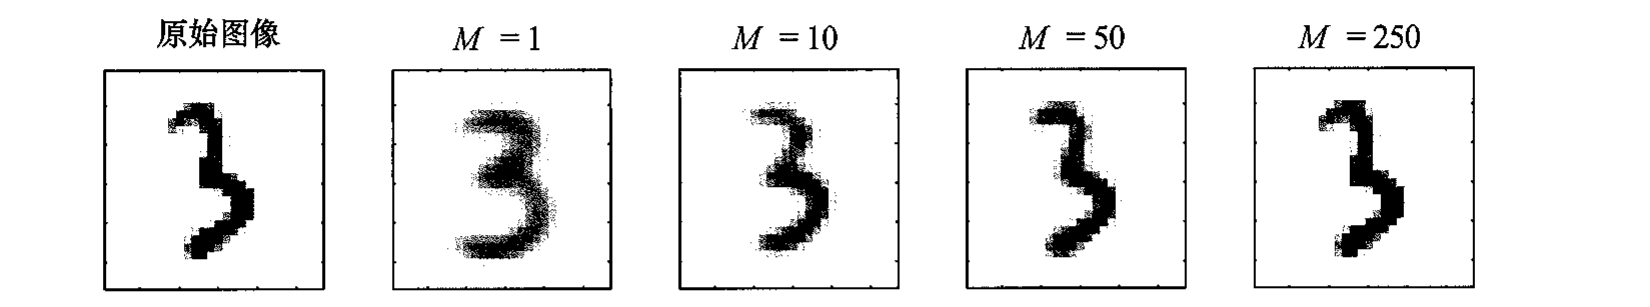
\includegraphics[width=0.95\textwidth]{ch16-fig16.5-pca-reconstruction.png}
  \caption{手写数字图像数据集中的一个手写数字及其通过保留 $M$ 个主成分而获得的 PCA 重构结果。随着 $M$ 值的增加，重构变得更准确，当 $M=D=28\times28=784$ 时，重构将会是完美的}
  \label{figure:ch16-PCA重建}
\end{figure}

\begin{remark}（重构新增）
压缩与重建是同一件事的两种说法：编码器把 $\bm{x}_n$ 映射为 $M$ 维码字 $\bm{z}_n=(\bm{x}_n-\bar{\bm{x}})^{\mathsf T}\bm{U}_M$，解码器用\eqref{align:ch16-重建}把它映回 $\tilde{\bm{x}}_n$。由于 $\bm{U}_M$ 的列正交归一，编码器是线性映射且不放大误差；又由\eqref{align:ch16-误差最小值}，重建的均方误差恰是被丢弃特征值之和，与码字分量无关。因此“保留 $M$ 个主成分”就是在给定码长的前提下使均方误差最小，而误差随 $M$ 的下降速度完全由特征值谱决定：谱衰减得越快，用很小的 $M$ 就能达到很小的误差，\cref{figure:ch16-特征值谱}给出的正是这一衰减曲线。
\end{remark}

\subsection{数据白化}\label{subsection:ch16-数据白化}

PCA 的另一个应用是数据预处理，其目标不是降低维度，而是转换数据集以标准化某些属性。变化后的数据集能更好地为机器学习算法服务。通常，当原始变量以不同的单位测量或具有显著不同的可变性时，就需要进行此类处理。例如，在老忠实喷泉数据集中，两次喷发之间的间隔时间通常比一次喷发的持续时间长一个数量级（见\cref{section:ch15-K均值聚类}）。将 $K$ 均值算法应用于这个数据集时，我们首先对各个变量进行了单独的线性重缩放，使得每个变量都具有零均值和单位方差。这称为标准化数据，标准化数据的协方差矩阵由以下元素构成：
\begin{align}
  \rho_{ij}=\frac{1}{N}\sum_{n=1}^{N}\frac{(x_{ni}-\bar{x}_i)}{\sigma_i}\frac{(x_{nj}-\bar{x}_j)}{\sigma_j},
  \label{align:ch16-相关系数}
\end{align}
其中 $\sigma_i$ 是 $x_i$ 的标准差。原始数据的相关性矩阵的特点是，如果数据的两个分量 $x_i$ 和 $x_j$ 完全相关，则 $\rho_{ij}=1$；如果它们不相关，则 $\rho_{ij}=0$。

利用 PCA，可以对数据进行更实质性的标准化，使其具有零均值和单位协方差，从而使不同的变量变得不相关。为此，首先将特征向量方程[\eqref{align:ch16-特征方程全}]写成以下形式：
\begin{align}
  \bm{S}\bm{U}=\bm{U}\bm{L},
  \label{align:ch16-特征分解}
\end{align}
其中 $\bm{L}$ 是一个 $D\times D$ 的对角矩阵，矩阵元素为 $\lambda_i$；$\bm{U}$ 是一个 $D\times D$ 的正交矩阵，其列由 $\bm{u}_i$ 给出。然后我们定义，对于每个数据点 $\bm{x}_n$，转换后的值由下式给出：
\begin{align}
  \bm{y}_n=\bm{L}^{-1/2}\bm{U}^{\mathsf T}(\bm{x}_n-\bar{\bm{x}}),
  \label{align:ch16-白化}
\end{align}
其中 $\bar{\bm{x}}$ 是由\eqref{align:ch16-均值}定义的样本均值。显然，集合 $\{\bm{y}_n\}$ 具有零均值，并且其协方差由单位矩阵给出，因为
\begin{align}
  \frac{1}{N}\sum_{n=1}^{N}\bm{y}_n\bm{y}_n^{\mathsf T}&=\frac{1}{N}\sum_{n=1}^{N}\bm{L}^{-1/2}\bm{U}^{\mathsf T}(\bm{x}_n-\bar{\bm{x}})(\bm{x}_n-\bar{\bm{x}})^{\mathsf T}\bm{U}\bm{L}^{-1/2}\nonumber\\
  &=\bm{L}^{-1/2}\bm{U}^{\mathsf T}\bm{S}\bm{U}\bm{L}^{-1/2}=\bm{L}^{-1/2}\bm{L}\bm{L}^{-1/2}=\bm{I}.
  \label{align:ch16-白化协方差}
\end{align}

\begin{definition}[白化]\label{definition:ch16-白化}
设 $\bm{S}=\bm{U}\bm{L}\bm{U}^{\mathsf T}$ 为数据协方差矩阵的特征分解，其中 $\bm{U}$ 正交、$\bm{L}$ 为对角矩阵且对角元 $\lambda_i>0$。称线性变换
\begin{align*}
  \bm{x}\mapsto\bm{y}=\bm{L}^{-1/2}\bm{U}^{\mathsf T}(\bm{x}-\bar{\bm{x}})
\end{align*}
为白化（whitening），也称球化（sphering）；变换后的数据集 $\{\bm{y}_n\}$ 称为白化数据。
\end{definition}

% SUPPLEMENT: parent=definition:ch16-白化; kind=motivation; location=紧随其后的 remark（重构新增）
\begin{remark}（重构新增）
白化把“标准化”从逐坐标的缩放推广为整体的线性变换。逐坐标标准化只令每个分量的方差为 $1$，并不消除分量之间的相关性（\eqref{align:ch16-相关系数}中的非对角元一般不为零）；白化则同时做到零均值、单位协方差，即各分量不相关且方差相同，因此数据的协方差形状被“揉成”一个球。

定义要求所有 $\lambda_i>0$。若某个 $\lambda_i=0$，$\bm{L}^{-1/2}$ 不存在，说明数据落在低维子空间里，此时只能在非零特征值对应的方向上白化，其余方向应删去（降维），这正是\cref{subsection:ch16-高维数据}讨论的情形。白化的代价是它依赖 $\bm{S}$ 的完整特征分解，复杂度为 $\mathcal{O}(D^3)$；当 $D$ 很大时通常先降维再白化。
\end{remark}

这个操作称为白化（whitening）或球化（sphering）数据，\cref{figure:ch16-白化}展示了对老忠实喷泉数据集（见\cref{section:ch15-K均值聚类}）应用线性预处理的效果。

\begin{figure}[htbp]
  \centering
  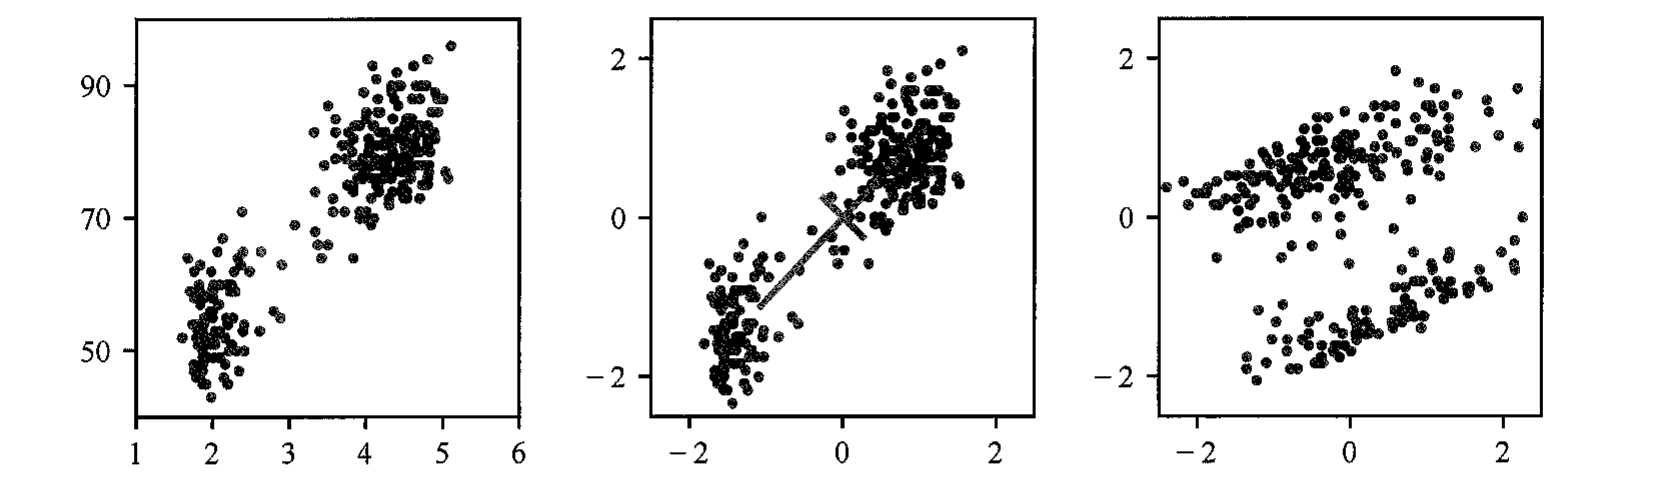
\includegraphics[width=0.95\textwidth]{ch16-fig16.6-whitening.png}
  \caption{对老忠实喷泉数据集应用线性预处理的效果。左图显示了原始数据。中图显示了将各个变量标准化为零均值和单位方差后的结果，同时显示了这个规范化数据集的主轴，它们绘制在范围 $\pm\lambda_i^{1/2}$ 内。右图显示了白化数据并得到零均值和单位协方差后的结果}
  \label{figure:ch16-白化}
\end{figure}

\subsection{高维数据}\label{subsection:ch16-高维数据}

在 PCA 的某些应用中，数据点的数量小于数据空间的维度。例如，我们可能想对一个有几百张图像的数据集应用 PCA，其中的每个图像对应于潜在的几百万维空间中的一个向量（对应于图像中每个像素的三个颜色值）。注意，在 $D$ 维空间中，$N$ 个点的集合（$N<D$）定义了一个线性子空间，其维度最多为 $N-1$，因此当 $M$ 的值大于 $N-1$ 时，应用 PCA 没有多大意义。实际上，如果我们执行 PCA，就会发现至少有 $D-N+1$ 个特征值是零，在这些特征值对应的特征向量方向上，数据的方差为零。

此外，寻找 $D\times D$ 矩阵的特征向量的典型算法的计算成本达到了 $\mathcal{O}(D^3)$ 的规模，因此对图像直接应用 PCA 在计算上是不可行的。

可以按照以下方式来解决这个问题。首先将 $\bm{X}$ 定义为 $N\times D$ 维的中心化数据矩阵，其第 $n$ 行由 $(\bm{x}_n-\bar{\bm{x}})^{\mathsf T}$ 给出。然后可以将协方差矩阵[\eqref{align:ch16-协方差}]写作 $\bm{S}=N^{-1}\bm{X}^{\mathsf T}\bm{X}$，相应的特征向量方程变为
\begin{align}
  \frac{1}{N}\bm{X}^{\mathsf T}\bm{X}\bm{u}_i=\lambda_i\bm{u}_i.
  \label{align:ch16-高维特征}
\end{align}

对\eqref{align:ch16-高维特征}的两边同时乘以 $\bm{X}$，得到
\begin{align}
  \frac{1}{N}\bm{X}\bm{X}^{\mathsf T}\left(\bm{X}\bm{u}_i\right)=\lambda_i\left(\bm{X}\bm{u}_i\right).
  \label{align:ch16-高维对偶}
\end{align}

如果定义 $\bm{v}_i=\bm{X}\bm{u}_i$，则可以得到
\begin{align}
  \frac{1}{N}\bm{X}\bm{X}^{\mathsf T}\bm{v}_i=\lambda_i\bm{v}_i.
  \label{align:ch16-高维v}
\end{align}

这是 $N\times N$ 矩阵 $N^{-1}\bm{X}\bm{X}^{\mathsf T}$ 的特征向量方程，它与原始协方差矩阵具有相同的 $N-1$ 个特征值（它本身还有额外的 $D-N+1$ 个特征值为零）。因此，我们可以在维度较低的空间中解决特征向量问题，计算成本为 $\mathcal{O}(N^3)$ 而不是 $\mathcal{O}(D^3)$。要确定特征向量，我们可以对\eqref{align:ch16-高维v}的两边乘以 $\bm{X}^{\mathsf T}$，得到
\begin{align}
  \left(\frac{1}{N}\bm{X}^{\mathsf T}\bm{X}\right)\left(\bm{X}^{\mathsf T}\bm{v}_i\right)=\lambda_i\left(\bm{X}^{\mathsf T}\bm{v}_i\right).
  \label{align:ch16-高维回代}
\end{align}

从中可以看出 $(\bm{X}^{\mathsf T}\bm{v}_i)$ 是具有特征值 $\lambda_i$ 的 $\bm{S}$ 的特征向量。但请注意，这些特征向量未必是归一化的。为了对它们进行适当的归一化，重新调整 $\bm{u}_i\propto\bm{X}^{\mathsf T}\bm{v}_i$，使得 $\|\bm{u}_i\|=1$（见\cref{exercise:ch16-03}），并且假设 $\bm{v}_i$ 已经归一化为单位长度，同时有
\begin{align}
  \bm{u}_i=\frac{1}{(N\lambda_i)^{1/2}}\bm{X}^{\mathsf T}\bm{v}_i.
  \label{align:ch16-高维归一化}
\end{align}

总之，要应用这种方法，我们需要首先计算 $\bm{X}\bm{X}^{\mathsf T}$，然后找到它的特征向量和特征值，最后使用\eqref{align:ch16-高维归一化}在原始数据空间中计算特征向量。

\begin{remark}（重构新增）
这一小节要解决的问题是“样本数少于维数”时 PCA 的可行性，包含两层困难。其一是统计上的：$N$ 个数据点至多张成 $N-1$ 维的子空间，因此当 $M\geqslant N$ 时，超出 $N-1$ 的那些“主成分”对应的方差恒为零，继续增加主成分数没有意义；这解释了为什么要求 $M\leqslant N-1$。其二是计算上的：$\bm{S}$ 是 $D\times D$ 矩阵，当 $D$ 达到百万量级时既无法存下也无法分解。

\eqref{align:ch16-高维对偶}—\eqref{align:ch16-高维v}给出的对偶技巧把问题从 $D\times D$ 转到 $N\times N$：$\bm{X}\bm{X}^{\mathsf T}$ 与 $\bm{X}^{\mathsf T}\bm{X}$ 的非零特征值完全相同（这是 $\bm{A}\bm{B}$ 与 $\bm{B}\bm{A}$ 的非零谱相同这一事实的特例），因此只需对 $N\times N$ 矩阵作特征分解，代价从 $\mathcal{O}(D^3)$ 降到 $\mathcal{O}(N^3)$。\eqref{align:ch16-高维归一化}中的因子 $(N\lambda_i)^{-1/2}$ 来自 $\|\bm{X}^{\mathsf T}\bm{v}_i\|^2=\bm{v}_i^{\mathsf T}\bm{X}\bm{X}^{\mathsf T}\bm{v}_i=N\lambda_i\bm{v}_i^{\mathsf T}\bm{v}_i=N\lambda_i$，这一步用了 $\bm{v}_i$ 已是单位向量以及\eqref{align:ch16-高维v}；若 $\lambda_i=0$ 则该方向无从归一化，这与“零方差方向”是同一件事。
\end{remark}

\end{document}
